The architecture of \emph{rmt} is quite simple and a diagram showing the architecture can be seen in figure \ref{fig:arch} which will be referred to throughout this section.

\begin{figure}[t]
	\centering
	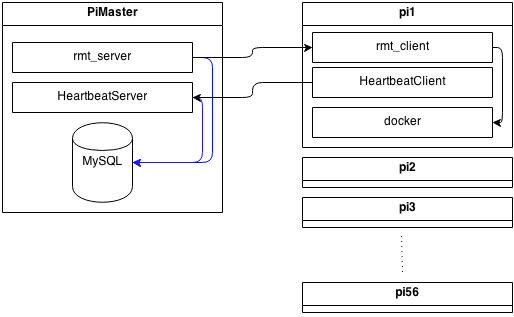
\includegraphics[width=0.6\textwidth]{rmtArch}
	\caption{diagram showing the architecture of \emph{rmt}}
	\label{fig:arch}
\end{figure}

\subsection{Overview}
The PiMaster has the \verb%rmt_server% application running which serves the web pages and retrieves data from the MySQL database and instances of \verb%rmt_client%.
PiMaster also has \verb%HeartbeatServer% running which listens on a specific port for messages from instances of \verb%HeartbeatClient%.

\verb%rmt_server% sends requests to \verb%rmt_client% via a REST interface for various pieces of information, the details of which are explained further in section [section reference].
Both \verb%rmt_server% and \verb%rmt_client% are web servers, the difference in names is to differentiate the server application from the application meant to be run on the hosts.

All of the Pi hosts have a software stack consisting of \verb%rmt_client%, \verb%HeartbeatClient%, and \verb%docker%.
There is no communication between \verb%rmt_client% and \verb%HeartbeatClient%.
\verb%rmt_client% and \verb%docker% communicate via a python wrapper module discussed in section \ref{impl:dockerpy}.

\subsection{Docker}
The docker module seen in the architecture diagram is docker running on the client.

\subsection{rmt\_client}
The name of this module is somewhat misleading in that it is not a client at all.
It is actually a \verb%web.py% application and therefore a web server, exposing the following RESTful [need some references for REST] interface.

\begin{description}
	\item[GET /cpu] returns a \verb%json% object corresponding to the cpu usage of the host in the same format as using \\\verb%psutil.cpu_times_percent%
	\item[GET /ram] returns a \verb%json% object corresponding to the ram usage of the host in bits
	\item[GET /temperature] returns a \verb%json% object containing a string with the temperature in [units]
	\item[GET /containers] returns a \verb%json% object containing the equivalent output to \verb%docker ps% which lists all currently running containers
	\item[GET /reboot] returns a \verb%json% object containing a message stating how many seconds it will be before a reboot takes place, and reboots the host
\end{description}

\subsection{MySQL Database}
Possibly include at least some of the creation script here.

\subsection{HeartbeatServer and HeartbeatClient}
Both of these are not original to \emph{rmt} as they were retrieved from [link] and this is stated as such in the comments of the source code.
However they were adapted for use in \emph{rmt}.

The HeartbeatServer component is listening on a particular (configurable) port for packets sent by HeartbeatClient.
Once these packets are received, the HeartbeatServer updates the sending host's corresponding last\_contacted field in the hosts table of the database with the current time.

\subsection{rmt\_server}
POSSIBLY SWAP PLACES WITH CLIENT AS IT MAY MAKE MORE SENSE...

In accordance with the \verb%web.py% framework \citep{webpy}, each web page is assigned a class and that class deals with the logic behind the request either by using the class's \verb%GET% or \verb%POST% method, depending on the type of HTTP request.
The functions not defined as \verb%GET% or \verb%POST% are not exposed via a web interface and are simply regular python functions, following regular python scoping rules.

For example, the \verb%add% class in \verb%rmt_server.py% has three functions: \verb%GET%, \verb%POST%, and \verb%try_host%.
In this example, \verb%try_host% is inaccessible from the web, but is used within the \verb%POST% method to error check the host address being added by the user.